\documentclass{article}
\usepackage{graphicx} % Required for inserting images
\usepackage{hyperref}
\usepackage{fancyvrb}
\usepackage[backend=biber, style=apa]{biblatex}
\addbibresource{references.bib}

% Set smaller font size for all Verbatim environments
\fvset{
  fontsize=\small
}

\title{Methodology for Predictive calculator}
\author{Anton Mukin}
\date{June 2025}

\setlength{\parindent}{0pt}


\begin{document}

\maketitle

\subsection{Brief Summary of the Project}
This Matura project investigates and evaluates the arithmetic capabilities 
of different neural networks. 

The project began with a literature review to 
generate a hypothesis regarding the weaknesses of neural networks in 
performing simple arithmetic. This literature review was submitted as the 
Zwischenprodukt, alongside a proof-of-concept notebook featuring a 
comparison of Feed-forward Neural Networks (FNNs) of different sizes.

The next step was to build a Recurrent Neural Network (RNN) and similar 
attention-based RNNs to investigate their arithmetic capabilities and 
compare them to those of the FNN using a benchmark.

The benchmark's baseline was defined to be the performance of a basic FNN's 
performance on different, but roughly still similar arithmetic tasks.

Afterwards, the same was done for the transformer type of neural network 
model. Here, their exact functionality was thuroughly investigated, because 
of their unique architectures.

Lastly a simillar workflow was repeated for some bigger, pre-trained models. 

And finally all the findings were collected and evaluated as a whole.


\subsection{Introduction to this document}
The goal of this document is assisting reproducability and showing how the 
findings discussed in the other document have been obtained.

All of the code written for this project is available in the github 
reporsitory: 

\url{https://github.com/AntonStantan/matura}

In this project all of the code is written in Python-notebooks (Jupyter Lab).
The preffered library used was \href{https://www.tensorflow.org/guide/keras}
{tensorflow keras}. 

Most of the models were trained locally on a Nvidia GPU device: \textit{Nvidia 
Jetson Orin Nano Super Developer Kit}

\begin{figure}[ht]
    \centering
    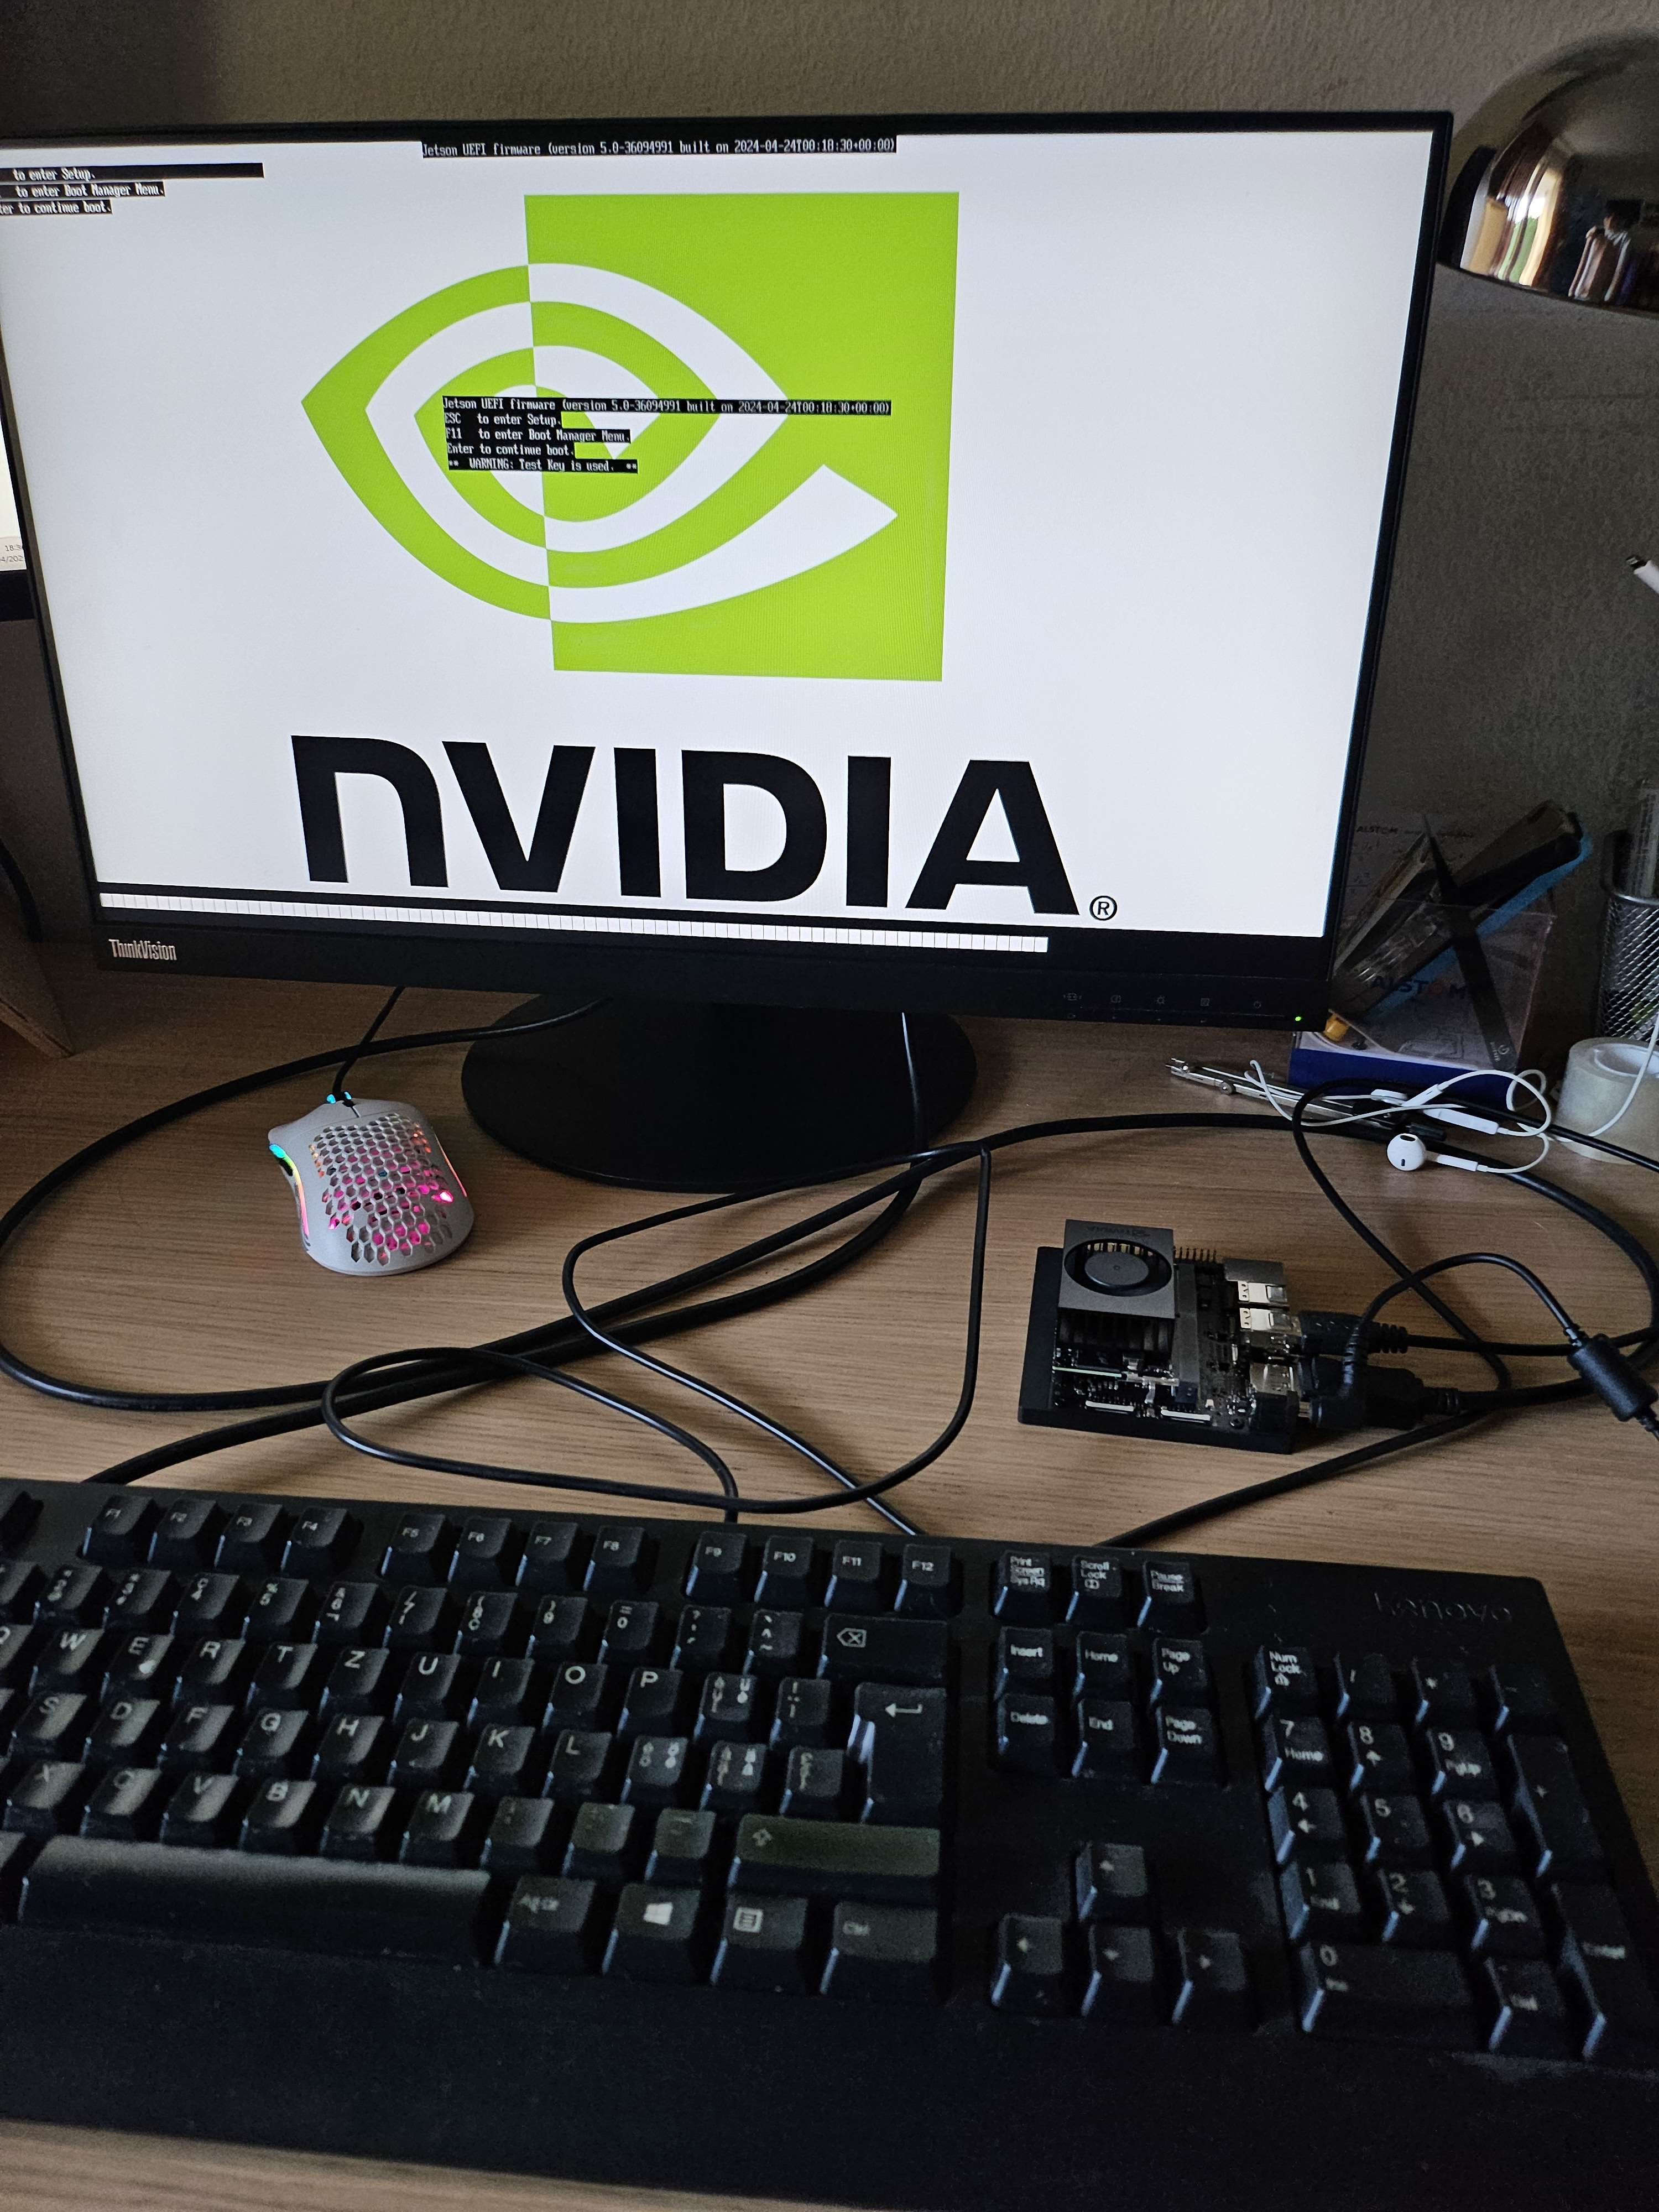
\includegraphics[width=0.5\paperwidth]{images/JetsonBoot.jpg}
    \caption{You can see the aformentioned Nvidia Jetson device booting up.}
    \label{fig:JetsonBoot}
\end{figure}

\newpage
\tableofcontents
\newpage

\section{Feed-forward Neural Networks (FNN)}
This section refers to the \href{https://github.com/AntonStantan/matura/tree/main/FNN}
{/FNN directory} in the github reporsitory.

There are two notebooks here: \href{https://github.com/AntonStantan/matura/blob/main/FNN/FNN1.ipynb}
{FNN1} and \href{https://github.com/AntonStantan/matura/blob/main/FNN/FNN2.ipynb}
{FNN2}.

\subsection{Train and Test data}
Defining the train data; The decision was made to only use subtraction and 
addition. The arithmetic expressions were defined to consist of two 
operators (+ or -) and three integers $[-5, 5]$

The reason for these definitions are: + and - are the 2 simplest operators. 
And the decision to introduce the model to 3 numbers, in place of the more 
commonly used 2, was made in hopes of simplifying the transition to more 
numbers later on.

e.g., the first three entries are: 
\[
1 - -2 + 3 \qquad -2 + -3 - -5 \qquad 3 - 1 - 0
\]
{\small In total there are 1907 expressions like this in the train data.}
\\[2em]
The test data is also defined in a slightly unconventional manner. It is 
split up into three categories.
\begin{itemize}
    \item Inside of the number range: Expressions just like in the train 
data but not inside of train data. 
    \item Outside of the number range: The same expressions, but with 
numbers in the ranges $[-8, -5]$ and $[5, 8]$ e.g.,
\[
-6 + 6 + 8 \qquad -7 + 6 + 7 \qquad 5 - -6 - 6
\]
    \item Longer expressions: Expressions of different lengths. 
Specifically, there are between 2 and 8 numbers inside of the $[-5, 5]$ 
range. e.g.,
\[
-5 + 1 \qquad 3 + -1 + 4 + -2 + -4 \qquad -2 + 1 + 5 + -5 - -2 + -1 - 2 - 5
\]
\end{itemize}

\subsection{Training a Neural Network Using Tensorflow}
This subsection will show how the models used in this project were first 
defined and then trained with tensorflow on the example of a simple FNN.
\\[2em]
To start of we will import the necessary libraries.
\begin{Verbatim}
import tensorflow as tf
from tensorflow import keras
from tensorflow.keras.layers import Dense, Layer, Dropout
from tensorflow.keras import layers, Sequential
from tensorflow.keras.layers import PReLU
\end{Verbatim}

And then we have to make a dataset out of the train and validation data 
discussed in the previous subsection. Let's use batches of 32.
Validation data is like the In-Range-test-data, except there aren't as many
expressions.
\begin{Verbatim}
batch_size = 32
train_dataset = tf.data.Dataset.from_tensor_slices((x_train, y_train))
.shuffle(len(x_train)).batch(batch_size)
val_dataset = tf.data.Dataset.from_tensor_slices((x_val, y_val))
.batch(batch_size)
\end{Verbatim}

We can now define the model using tf.keras.Sequential. The model's 
architecture is clearly visible. In this example the model has two dense 
layers with 64 neurons each.

The activation function used is PReLU, as this is the one, which was the  
most promising in \cite{trask2018neuralarithmeticlogicunits}. 

Drop-out is included to prevent overfitting. In most models used in this 
project it wasn't necessary.

As you can see, the input-shape has to be defined, when defining the model.

Additionally, please notice how the output layer only consists of a single 
neuron with a linear activation function. This means the model we just 
created is a regression model. This is similar to not having a decoder.
\begin{Verbatim}
input_shape = (15,)
model = Sequential([
    keras.Input(shape = input_shape),     #input

    Dense(64),                            #first dense layer
    PReLU(),                              #PReLU activation function
    Dropout(0.1),                         #dropout layer

    Dense(64),                            #second dense layer
    PReLU(),                                
    Dropout(0.1),                           

    Dense(1, activation='linear')         #output layer
])
\end{Verbatim}

The next step is to compile the model, by choosing an optimizer and loss 
calculation e.g., in our case Mean Squared Error (MSE)
\begin{Verbatim}
model.compile(optimizer="adam", loss="mse")
\end{Verbatim}

The last step remaining is to fit the model on some data. We will be 
fitting our model on the previously defined train and validation data. 
The training process will take 200 epochs to complete or it might be aborted
preemtively if the model starts to overfit and early\_stopping is triggered.

\begin{Verbatim}
model.fit(
    train_dataset,
    validation_data=val_dataset,
    epochs=200,
    callbacks=[early_stopping],
    verbose=1
)
\end{Verbatim}

\subsection{FNN1 and FNN2 Notebooks}
In this project two notebooks with FNNs have been created. FNN1 and FNN2. 
In FNN1 a simple FNN was created, it's performance was evaluated and FNNs 
of different sizes have been compared against eachother in a heatmap. It is 
noteworthy, that the models here have been used with a bootstrap, meaning 
multiple models with the same sizes were trained and then used to give one 
combined prediction. This was done to reduce noise. In later notebooks this 
will not be the case, as this makes it more difficult to accurately evaluate 
a model.
\\[2em]
FNN2 includes a model with hyperparameters (in this case the number of 
neurons, the number of layers and whether or not to use dropout) chosen by 
the keras-tuner. This is simply put an automatization: It picks out models 
with different hyperparameters, trains them and compares their performance 
on validation data. The model with the best-performing hyperparameters will 
be chosen as the best model.

The model in FNN2 is evaluated inside of that notebook and it's benchmark 
is calculated.

\subsection{The Benchmark}


\subsection{Drop-Out}
When introducing a Drop-Out with an industry standard value of 0.3; contrary 
to the expectation of reducing over-fitting, which in some way is present, 
as the models aren't able to generalize beyond the training range, this has 
a negative effect on the model. The MSEs of models with Drop-out are higher 
then, the ones of the previous models without drop-out.
% https://github.com/AntonStantan/matura/blob/main/FNN_Heatmaps/DropOutComparison.png
%this is kinda wrong. Will explain later

\section{Recurrent Neural Network (RNN)}
\subsection{Introduction}
Recurrent Neural Networks (RNNs) work similar to FNNs with one key 
difference: There is a vector called the hidden-state. This vector contains 
information about previous inputs. The hidden-state of the previous 
time-step, in addition to the input of the current time-step, is fed into a 
model which computes the hidden-state of the present time-step. The output 
of each time-step is calculated by feeding the respective hiddenstate to a 
model.

\newpage
\textbf{ Numerical Visualization:}


Let:
\begin{itemize}
    \item $x_t$: Input at time step $t$
    \item $h_t$: Hidden state at time step $t$
    \item $y_t$: Output at time step $t$
    \item $W_{xh}$: Weight matrix connecting input to hidden state
    \item $W_{hh}$: Weight matrix connecting previous hidden state to current hidden state (recurrent weights)
    \item $W_{hy}$: Weight matrix connecting hidden state to output
    \item $b_h$: Bias vector for the hidden layer
    \item $b_y$: Bias vector for the output layer
    \item $\sigma$: Activation function (commonly tanh or ReLU for the hidden state)
    \item $\sigma_{out}$: Activation function for the output (e.g. softmax for classification, or linear in our case of regression)
\end{itemize}



$$h_t = \sigma(W_{xh}x_t + W_{hh}h_{t-1} + b_h)$$

$$y_t = \sigma_{out}(W_{hy}h_t + b_y)$$



Useful sources for the creation of the first RNN prototype:
% https://www.ibm.com/think/topics/recurrent-neural-networks
% https://arxiv.org/pdf/1406.1827
% https://www.tensorflow.org/guide/keras/working_with_rnns
\newpage

%\section{attention}

%https://arxiv.org/abs/1409.0473
%https://arxiv.org/abs/1508.04025
%https://www.tensorflow.org/api_docs/python/tf/keras/layers/Attention


\printbibliography[heading=bibintoc]

\end{document}
